Há três tipos de ambientes no desenvolvimento desta aplicação: \textit{development}, \textit{staging} e \textit{production}. O ambiente de \textit{development}, ou desenvolvimento, é o ambiente local de cada desenvolvedor, \textit{staging} ou pré produção é um ambiente para serem realizados testes beta e \textit{production} ou produção é o ambiente final onde a aplicação será de fato utilizada pelos usuários.

Na API a integração contínua é feita com a ferramenta TravisCI. Onde, se um \textit{pull request} é aceito na \textit{branch} \textit{staging}, o Travis executa toda a suíte de testes para ver se algum deles pode ter resultado em falha. Caso todos passem, ele verifica se todas as métricas definidas pelo Rubocop estão de acordo com o padrão definido. Caso todas as métricas passem, a \textit{build} de pré produção é criada, o Travis envia as informações de cobertura de testes para o Coveralls, as informações de métricas para o Code Climate e logo em seguida realiza o \textit{deploy} no ambiente de pré produção no Heroku.

Se um \textit{pull request} for aceito na \textit{branch} \textit{master} todo o processo será o mesmo, com exceção que o \textit{deploy} irá ocorrer no ambiente de produção no Heroku.

A Figura \ref{img:integracao_deploy_continuo_api} ilustra o processo de integração e \textit{deploy} contínuo feito na API.

\begin{figure}[H]
    \centering
    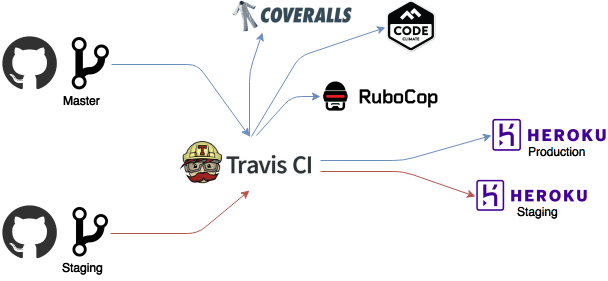
\includegraphics[scale=0.5]{figuras/api_ci.png}
    \caption[Integração e \textit{deploy} contínuo API]{Integração e \textit{deploy} contínuo API. Fonte: autores}
    \label{img:integracao_deploy_continuo_api}
\end{figure}

No aplicativo foi planejada a integração e o \textit{deploy} contínuo para ocorrer como mostra a Figura \ref{img:integracao_deploy_continuo_planejado_app}.

\begin{figure}[H]
    \centering
    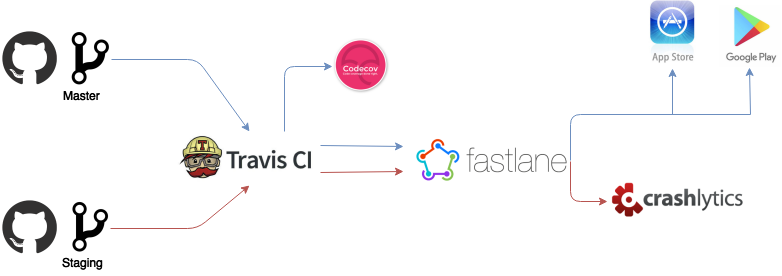
\includegraphics[scale=0.5]{figuras/ci_should_be.png}
    \caption[Integração e \textit{deploy} contínuo planejado para o aplicativo]{Integração e \textit{deploy} contínuo planejado para o aplicativo. Fonte: autores}
    \label{img:integracao_deploy_continuo_planejado_app}
\end{figure}

Se um \textit{pull request} é aceito na \textit{branch} \textit{master}, o Travis irá realizar toda a suíte de testes, caso todos passem enviará as informações de cobertura para o
Codecov e através do Fastlane realizará o \textit{deploy} do aplicativo tanto na Play Store quanto na App Store. E se um \textit{pull request} for aceito na \textit{branch} \textit{staging}, todo o processo é repetido, exceto quando não é realizado o \textit{deploy} do aplicativo nas lojas e sim no Crashlytics, que irá criar a versão beta do aplicativo e o enviará para os emails configurados previamente.

Uma vez que o aplicativo ainda não chegou ao estágio de \textit{deploy} nas lojas, o planejamento para a primeira entrega é só até o \textit{deploy} beta, como mostrado na Figura \ref{img:integracao_deploy_continuo_planejado_primeira_entrega}:

\begin{figure}[H]
    \centering
    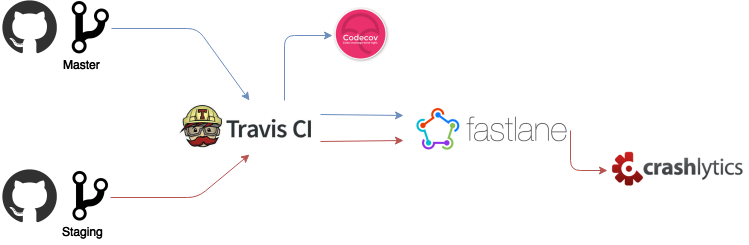
\includegraphics[scale=0.5]{figuras/ci_as_is.png}
    \caption[Integração e \textit{deploy} contínuo planejado para a primeira entrega]{Integração e \textit{deploy} contínuo planejado para a primeira entrega. Fonte: autores}
    \label{img:integracao_deploy_continuo_planejado_primeira_entrega}
\end{figure}

Entretanto, não foi possível fazer com que o \textit{deploy} contínuo aconteça logo após a integração contínua, um desafio causado por escolher desenvolvimento híbridos de aplicativo. Uma vez que o código versionado do aplicativo é o mesmo código para a plataforma Android e iOS, e após realizar a \textit{build} desse código é gerado códigos em cada plataforma (não versionados). A ferramenta de integração contínua não consegue ter acesso aos códigos de cada plataforma para realizar os devidos \textit{deploys}. Sendo assim, o \textit{deploy} contínuo está acontecendo manualmente, por enquanto, até que solução seja encontrada, através do comando:

\begin{lstlisting}[language=bash]
  $ fastlane beta
\end{lstlisting}

Sendo assim, a Figura \ref{img:integracao_deploy_continuo_atual} ilustra como está funcionando a integração e o \textit{deploy} contínuo do aplicativo até o presente momento.

\begin{figure}[H]
    \centering
    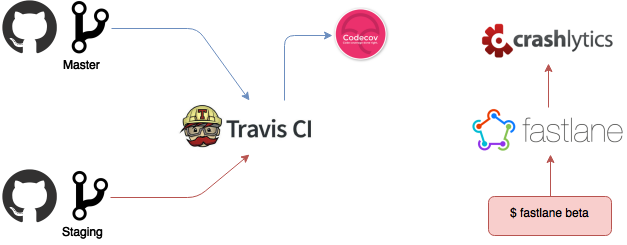
\includegraphics[scale=0.5]{figuras/ci_currently.png}
    \caption[Integração e \textit{deploy} contínuo atual]{Integração e \textit{deploy} contínuo atual. Fonte: autores}
    \label{img:integracao_deploy_continuo_atual}
\end{figure}
